\section{Feldbilder}
Um eine weitgehendere Analyse der Auswirkung von Kurzschl\"ussen zu f\"uhren, k\"onnen aus CST Feldbilder ausgelesen werden. Diese zeigen, in wie weit das magnetische Feld durch die Kurzschl\"usse aus dem inneren des MA-Ringkerns verdr\"angt wird. Dazu werden einige Kurzschlussanordnungen gegen\"uber gestellt. Zun\"achst wird der Einfluss eines einzigen Kurzschlusses mit der Breite $\SI{30}{\milli\meter}$, der Länge $\SI{160}{\milli\meter}$ sowie einer Blechdicke von $\SI{1}{\milli\meter}$ gegen\"uber dem reinen Ringkern ohne Kurzschl\"usse nach Abbildung~\ref{fig:0zu1ks} betrachtet.


\newpage



\begin{figure}[htb]
	\centering
	\subfloat[Ringkern Ohne Kurzschl\"usse]{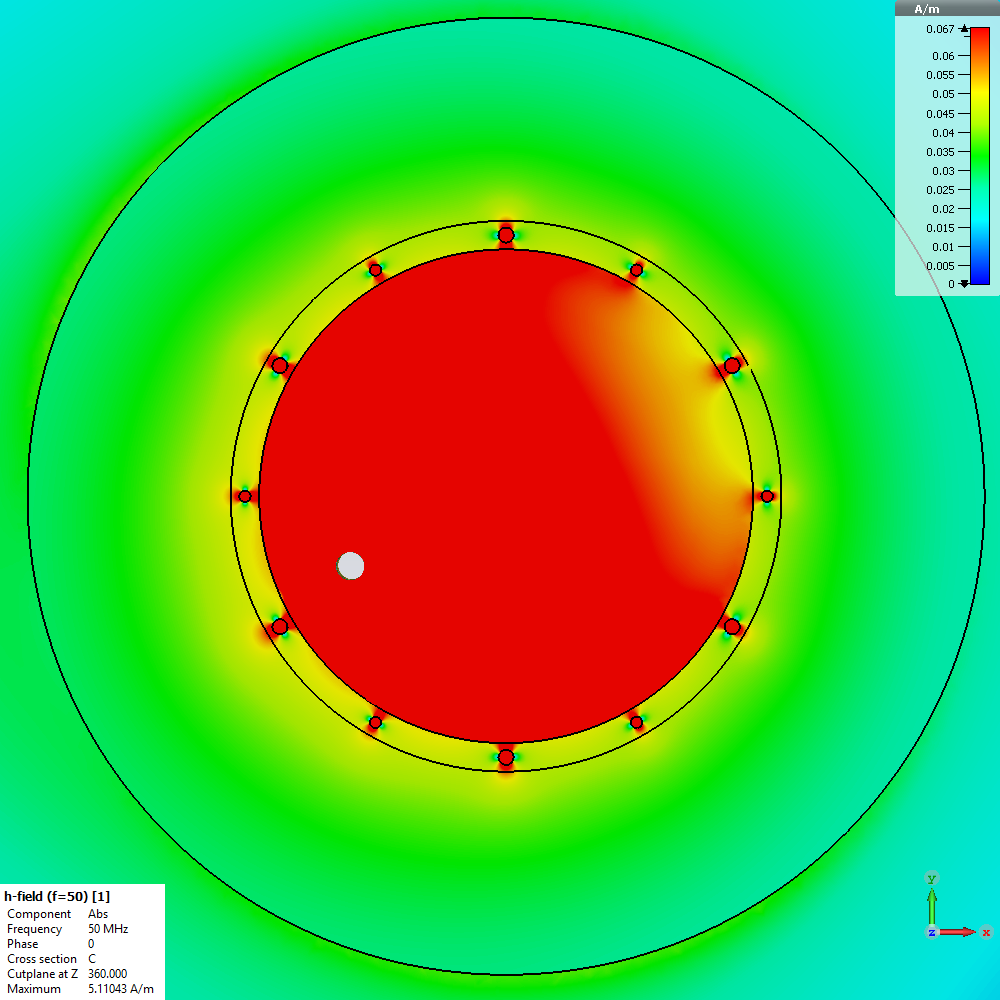
\includegraphics[width=0.45\textwidth]{Feldbilder/0KS}}
	\hspace{0.03\textwidth}
	\subfloat[Ringkern mit einem Kurzschluss der Breite $\SI{30}{\milli\meter}$ und der Länge $\SI{160}{\milli\meter}$.]{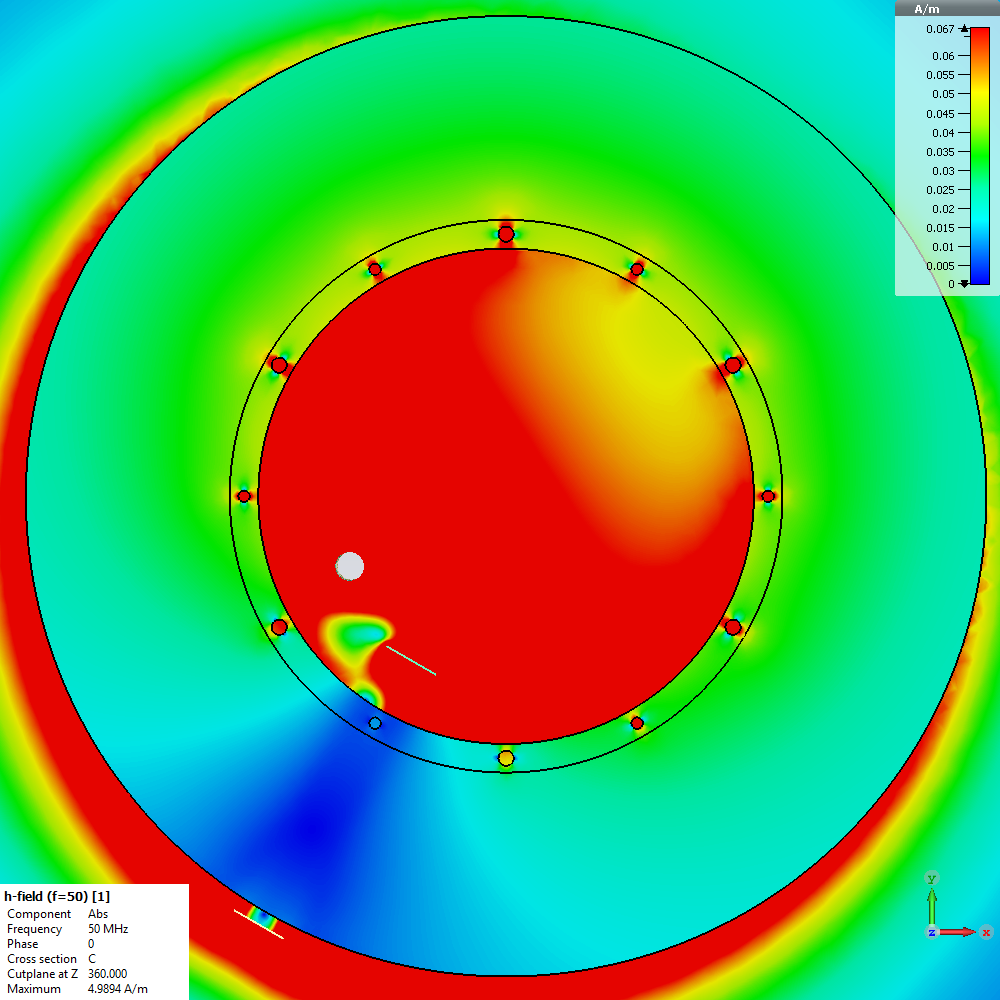
\includegraphics[width=0.45\textwidth]{Feldbilder/1KS}}
	\caption{Gegen\"uberstellung der Feldverteilung des Magnetischen Feldes innerhalb des Ringkerns ohne Kurzschluss und mit einem Kurzschluss.}
	\label{fig:0zu1ks}
\end{figure}
\par
Bereits ein Kurzschluss verd\"angt schon einen gro\ss{}en Teil des magnetischen Feldes. Dieser Effekt ist in dem Bereich des Ringkerns, welcher von der Kurzschlusschiene \"uberdeckt ist, oder in der n\"ahe liegt deutlich st\"arker als in anderen Ringkernregionen. Dieser Effekt ist auch bei einer h\"oheren Anzahl an Kurzschl\"ussen sichtbar. Abbildung~\ref{fig:1zu8ks} zeigt den Vergleich von einem Kurzschluss zur maximalen Anzahl von acht Kurzschl\"ussen.
\begin{figure}[htb]
	\centering
	\subfloat[Ringkern mit einem Kurzschluss der Breite $\SI{30}{\milli\meter}$ und der Länge $\SI{160}{\milli\meter}$.]{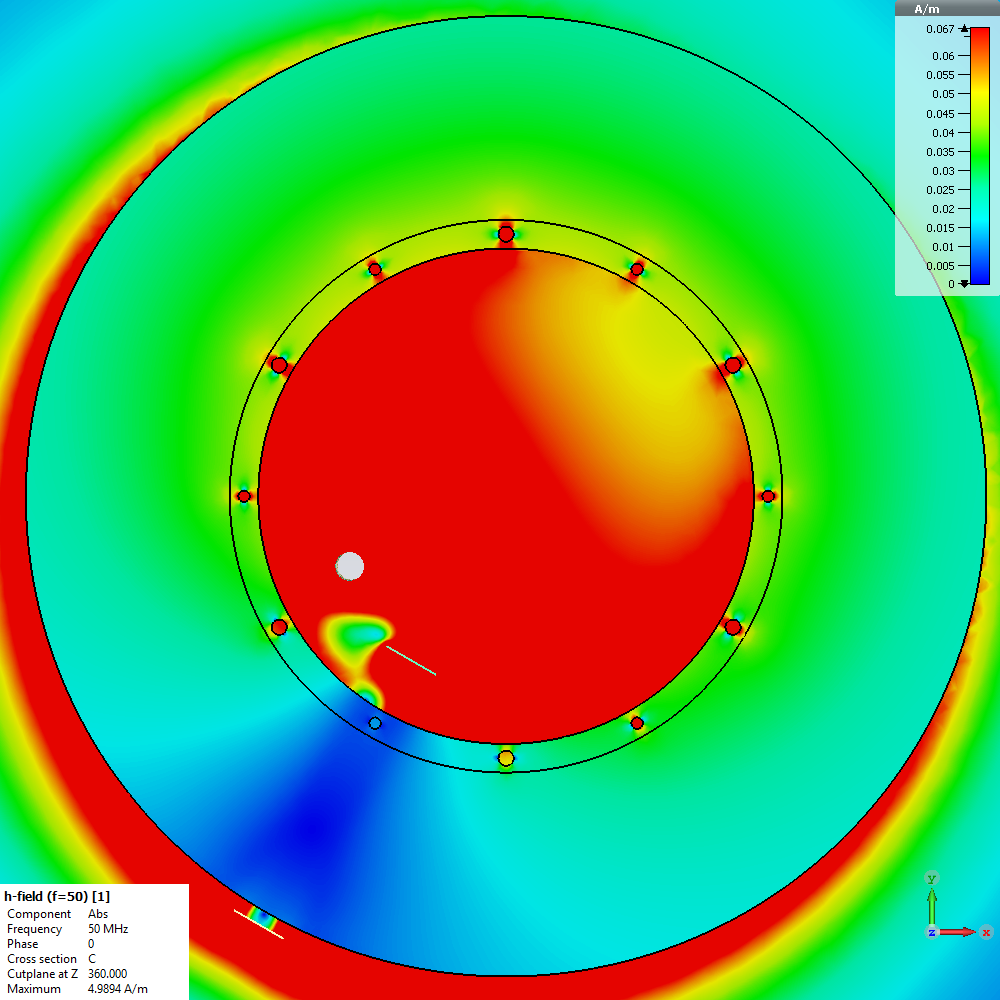
\includegraphics[width=0.45\textwidth]{Feldbilder/1KS}}
	\hspace{0.03\textwidth}
	\subfloat[Ringkern mit acht Kurzschl\"ussen der Breite $\SI{30}{\milli\meter}$ und der Länge $\SI{160}{\milli\meter}$.]{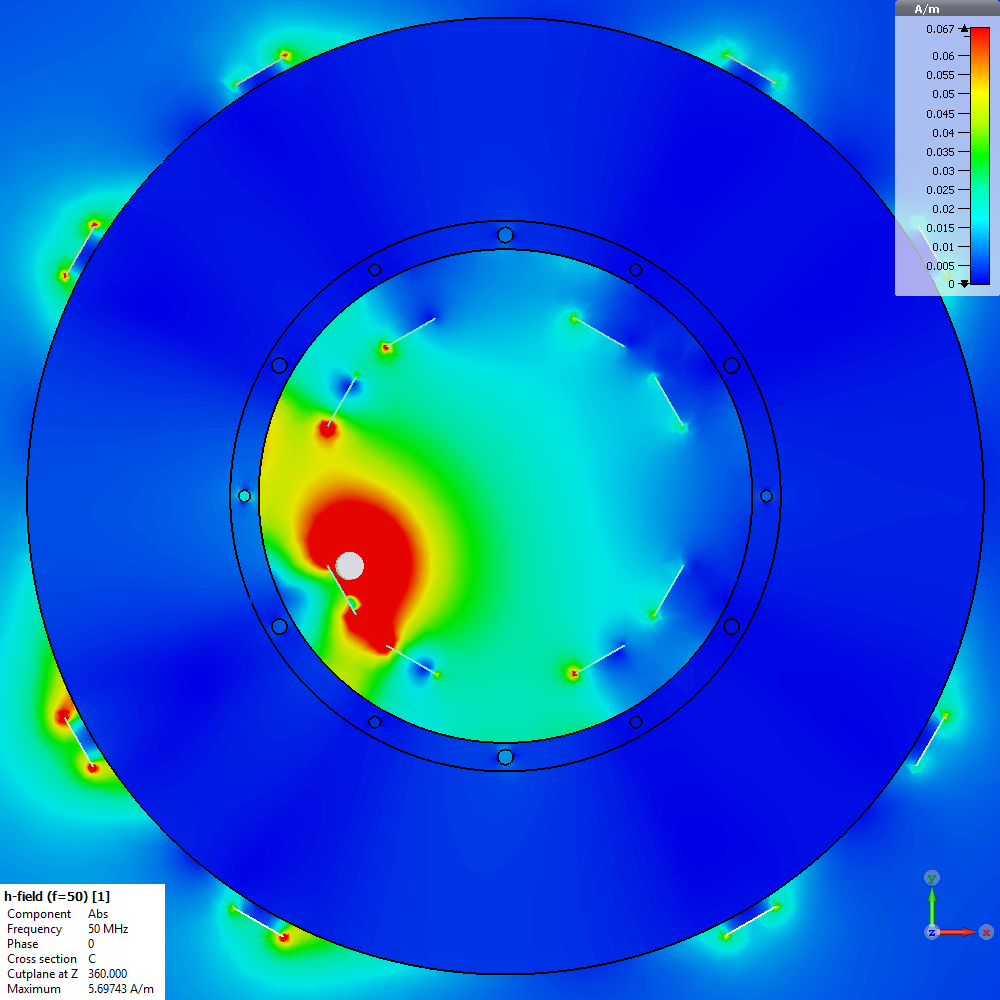
\includegraphics[width=0.45\textwidth]{Feldbilder/8KS}}
	\caption{Gegen\"uberstellung der Feldverteilung des Magnetischen Feldes innerhalb des Ringkerns mit einem Kurzschluss und mit acht Kurzschl\"ussen.}
	\label{fig:1zu8ks}
\end{figure}
\par
Die Beobachtung liefert auch eine Erkl\"arung, warum zwei schmale Kurzschl\"usse eine st\"arkere Verringerung der Ringkernimpedanz nach sich ziehen, als ein breiter Kurzschluss. Da das Feld besonders im Umkreis des Kurzschlusses geringer ist, f\"uhrt eine weitere Verteilung der Kurzschl\"usse zu geringeren Feldst\"arken im gesamten Ring. Dieser Effekt ist in Abbildung~\ref{fig:150zu220ks} zu sehen. 
\begin{figure}[htb]
	\centering
	\subfloat[Ringkern mit einem Kurzschluss der Breite $\SI{50}{\milli\meter}$ und der Länge $\SI{160}{\milli\meter}$.]{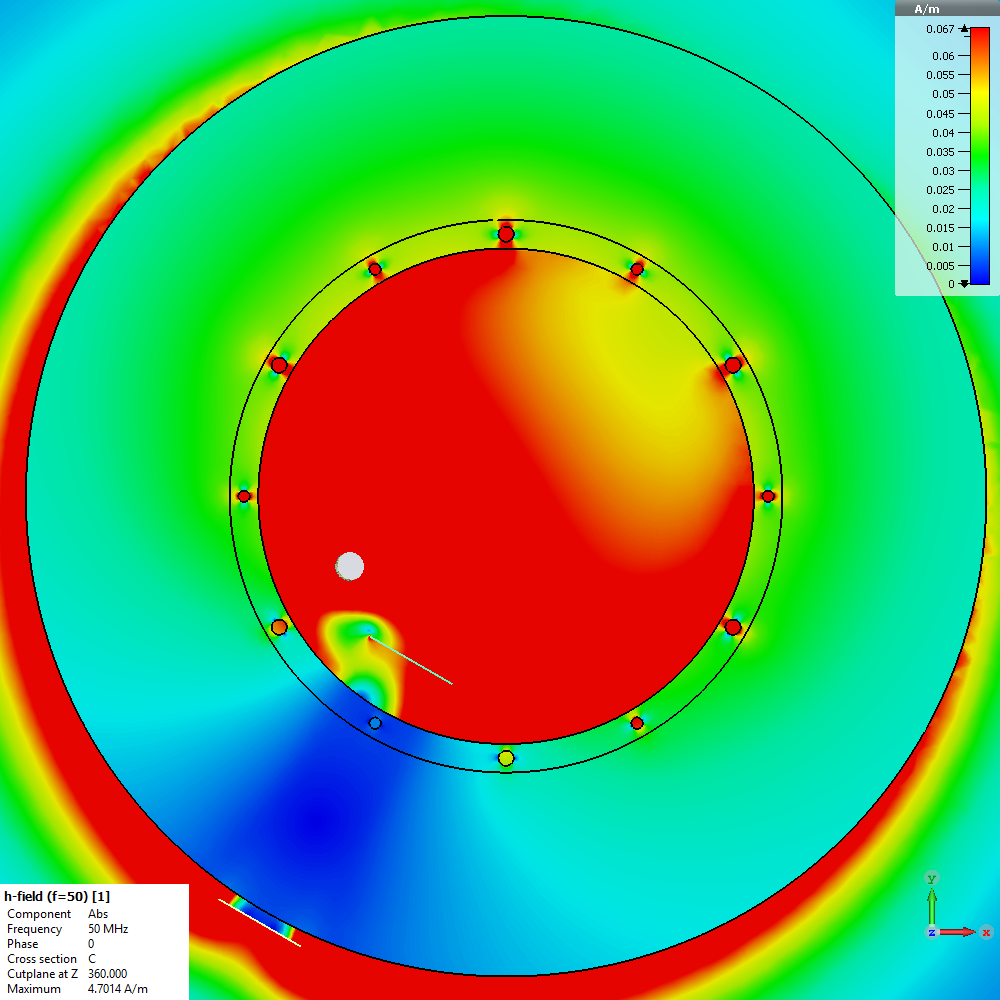
\includegraphics[width=0.45\textwidth]{Feldbilder/1KSb50}}
	\hspace{0.03\textwidth}
	\subfloat[Ringkern mit zwei Kurzschl\"ussen der Breite $\SI{20}{\milli\meter}$ und der Länge $\SI{160}{\milli\meter}$.]{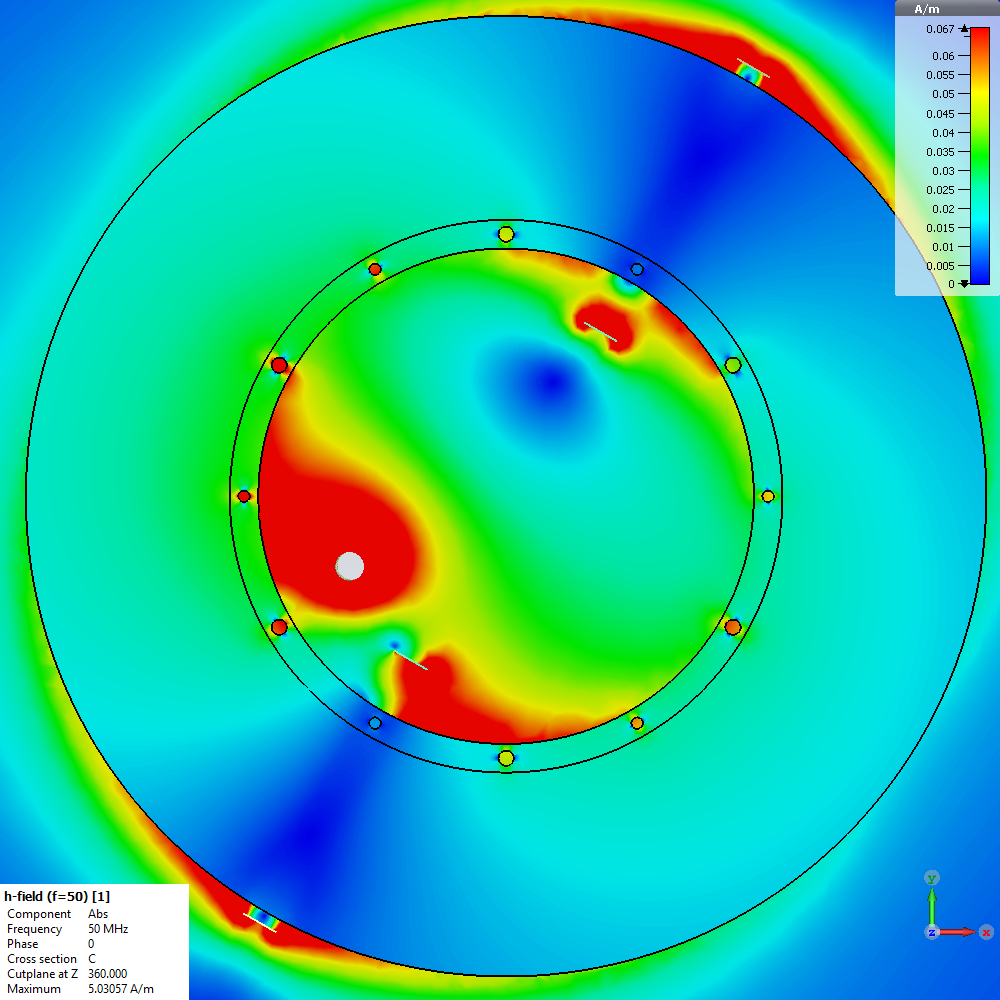
\includegraphics[width=0.45\textwidth]{Feldbilder/2KSb20}}
	\caption{Gegen\"uberstellung der Feldverteilung des Magnetischen Feldes innerhalb des Ringkerns mit einem Kurzschluss der Breite $\SI{50}{\milli\meter}$ und mit zwei Kurzschl\"ussen der Breite $\SI{20}{\milli\meter}$.}
	\label{fig:150zu220ks}
\end{figure}
\par
Wird vorausgesetzt, dass die Ringkernimedanz direkt mit dem mittleren Feld zusammenh\"angt, so dient dies als eine plausible Erkl\"arung f\"ur bisher beobachtete Effekte. Die Komplette Ansicht der Feldverteilung f\"ur alle Kurzschlussanordnungen ist in Anhang~\ref{sec:allfieldplots} gegeben.